% Created 2024-12-22 So 15:24
% Intended LaTeX compiler: lualatex
\documentclass{mimosis}
                  \usepackage[hyperref,x11names]{xcolor}
\usepackage[
colorlinks = true,
citecolor  = RoyalBlue,
linkcolor  = RoyalBlue,
urlcolor   = RoyalBlue,
unicode
]{hyperref}
\usepackage{fontspec}
\usepackage{ltablex}
\usepackage{unicode-math}
\setmonofont{DejaVu Sans Mono}[Scale=0.8]
\newenvironment{abstract} {}{}
\usepackage{abstract}
\usepackage{multicol}
\usepackage{supertabular,booktabs}
\DeclareMathOperator*{\argmax}{arg\,\max}
\usepackage{booktabs}
\usepackage{multicol}
\usepackage{siunitx}
\newenvironment{multicoltable}[1][3]{\begin{multicols}{#1}\begin{supertabular}}{\end{supertabular}\end{multicols}}

%% ox-latex features:
%   !announce-start, bibliography-biblatex, !guess-pollyglossia, !guess-babel,
%   !guess-inputenc, engraved-code, caption, image,
%   bibliography-biblatex-resources, !announce-end.

\usepackage{biblatex}


% Setup for code blocks [1/2]

\usepackage{fvextra}

\fvset{%
  commandchars=\\\{\},
  highlightcolor=white!95!black!80!blue,
  breaklines=true,
  breaksymbol=\color{white!60!black}\tiny\ensuremath{\hookrightarrow}}

% Make line numbers smaller and grey.
\renewcommand\theFancyVerbLine{\footnotesize\color{black!40!white}\arabic{FancyVerbLine}}

\usepackage{xcolor}

% In case engrave-faces-latex-gen-preamble has not been run.
\providecolor{EfD}{HTML}{f7f7f7}
\providecolor{EFD}{HTML}{28292e}

% Define a Code environment to prettily wrap the fontified code.
\usepackage[breakable,xparse]{tcolorbox}
\providecommand{\codefont}{\footnotesize}
\DeclareTColorBox[]{Code}{o}%
{colback=EfD!98!EFD, colframe=EfD!95!EFD,
  fontupper=\setlength{\fboxsep}{0pt}\codefont,
  colupper=EFD,
  IfNoValueTF={#1}%
  {boxsep=2pt, arc=2.5pt, outer arc=2.5pt,
    boxrule=0.5pt, left=2pt}%
  {boxsep=2.5pt, arc=0pt, outer arc=0pt,
    boxrule=0pt, leftrule=1.5pt, left=0.5pt},
  right=2pt, top=1pt, bottom=0.5pt,
  breakable}

% Support listings with captions
\usepackage{float}
\floatstyle{plain}
\newfloat{listing}{htbp}{lst}
\newcommand{\listingsname}{Listing}
\floatname{listing}{\listingsname}
\newcommand{\listoflistingsname}{List of Listings}
\providecommand{\listoflistings}{\listof{listing}{\listoflistingsname}}


% Setup for code blocks [2/2]: syntax highlighting colors

\newcommand\efstrut{\vrule height 2.1ex depth 0.8ex width 0pt}
\definecolor{EFD}{HTML}{000000}
\definecolor{EfD}{HTML}{ffffff}
\newcommand{\EFD}[1]{\textcolor{EFD}{#1}} % default
\definecolor{EFvp}{HTML}{000000}
\newcommand{\EFvp}[1]{\textcolor{EFvp}{#1}} % variable-pitch
\definecolor{EFh}{HTML}{7f7f7f}
\newcommand{\EFh}[1]{\textcolor{EFh}{#1}} % shadow
\definecolor{EFsc}{HTML}{228b22}
\newcommand{\EFsc}[1]{\textcolor{EFsc}{\textbf{#1}}} % success
\definecolor{EFw}{HTML}{ff8e00}
\newcommand{\EFw}[1]{\textcolor{EFw}{\textbf{#1}}} % warning
\definecolor{EFe}{HTML}{ff0000}
\newcommand{\EFe}[1]{\textcolor{EFe}{\textbf{#1}}} % error
\definecolor{EFl}{HTML}{ff0000}
\newcommand{\EFl}[1]{\textcolor{EFl}{#1}} % link
\definecolor{EFlv}{HTML}{ff0000}
\newcommand{\EFlv}[1]{\textcolor{EFlv}{#1}} % link-visited
\definecolor{EFhi}{HTML}{ff0000}
\newcommand{\EFhi}[1]{\textcolor{EFhi}{#1}} % highlight
\definecolor{EFc}{HTML}{b22222}
\newcommand{\EFc}[1]{\textcolor{EFc}{#1}} % font-lock-comment-face
\definecolor{EFcd}{HTML}{b22222}
\newcommand{\EFcd}[1]{\textcolor{EFcd}{#1}} % font-lock-comment-delimiter-face
\definecolor{EFs}{HTML}{8b2252}
\newcommand{\EFs}[1]{\textcolor{EFs}{#1}} % font-lock-string-face
\definecolor{EFd}{HTML}{8b2252}
\newcommand{\EFd}[1]{\textcolor{EFd}{#1}} % font-lock-doc-face
\definecolor{EFm}{HTML}{008b8b}
\newcommand{\EFm}[1]{\textcolor{EFm}{#1}} % font-lock-doc-markup-face
\definecolor{EFk}{HTML}{9370db}
\newcommand{\EFk}[1]{\textcolor{EFk}{#1}} % font-lock-keyword-face
\definecolor{EFb}{HTML}{483d8b}
\newcommand{\EFb}[1]{\textcolor{EFb}{#1}} % font-lock-builtin-face
\definecolor{EFf}{HTML}{0000ff}
\newcommand{\EFf}[1]{\textcolor{EFf}{#1}} % font-lock-function-name-face
\definecolor{EFv}{HTML}{a0522d}
\newcommand{\EFv}[1]{\textcolor{EFv}{#1}} % font-lock-variable-name-face
\definecolor{EFt}{HTML}{228b22}
\newcommand{\EFt}[1]{\textcolor{EFt}{#1}} % font-lock-type-face
\definecolor{EFo}{HTML}{008b8b}
\newcommand{\EFo}[1]{\textcolor{EFo}{#1}} % font-lock-constant-face
\definecolor{EFwr}{HTML}{ff0000}
\newcommand{\EFwr}[1]{\textcolor{EFwr}{\textbf{#1}}} % font-lock-warning-face
\newcommand{\EFnc}[1]{#1} % font-lock-negation-char-face
\definecolor{EFpp}{HTML}{483d8b}
\newcommand{\EFpp}[1]{\textcolor{EFpp}{#1}} % font-lock-preprocessor-face
\newcommand{\EFrc}[1]{\textbf{#1}} % font-lock-regexp-grouping-construct
\newcommand{\EFrb}[1]{\textbf{#1}} % font-lock-regexp-grouping-backslash
\newcommand{\EFob}[1]{#1} % org-block
\newcommand{\EFobb}[1]{#1} % org-block-begin-line
\newcommand{\EFobe}[1]{#1} % org-block-end-line
\definecolor{EFOa}{HTML}{0000ff}
\newcommand{\EFOa}[1]{\textcolor{EFOa}{#1}} % outline-1
\definecolor{EFOb}{HTML}{a0522d}
\newcommand{\EFOb}[1]{\textcolor{EFOb}{#1}} % outline-2
\definecolor{EFOc}{HTML}{a020f0}
\newcommand{\EFOc}[1]{\textcolor{EFOc}{#1}} % outline-3
\definecolor{EFOd}{HTML}{b22222}
\newcommand{\EFOd}[1]{\textcolor{EFOd}{#1}} % outline-4
\definecolor{EFOe}{HTML}{228b22}
\newcommand{\EFOe}[1]{\textcolor{EFOe}{#1}} % outline-5
\definecolor{EFOf}{HTML}{008b8b}
\newcommand{\EFOf}[1]{\textcolor{EFOf}{#1}} % outline-6
\definecolor{EFOg}{HTML}{483d8b}
\newcommand{\EFOg}[1]{\textcolor{EFOg}{#1}} % outline-7
\definecolor{EFOh}{HTML}{8b2252}
\newcommand{\EFOh}[1]{\textcolor{EFOh}{#1}} % outline-8
\definecolor{EFhn}{HTML}{008b8b}
\newcommand{\EFhn}[1]{\textcolor{EFhn}{#1}} % highlight-numbers-number
\definecolor{EFhq}{HTML}{9370db}
\newcommand{\EFhq}[1]{\textcolor{EFhq}{#1}} % highlight-quoted-quote
\definecolor{EFhs}{HTML}{008b8b}
\newcommand{\EFhs}[1]{\textcolor{EFhs}{#1}} % highlight-quoted-symbol
\definecolor{EFrda}{HTML}{707183}
\newcommand{\EFrda}[1]{\textcolor{EFrda}{#1}} % rainbow-delimiters-depth-1-face
\definecolor{EFrdb}{HTML}{7388d6}
\newcommand{\EFrdb}[1]{\textcolor{EFrdb}{#1}} % rainbow-delimiters-depth-2-face
\definecolor{EFrdc}{HTML}{909183}
\newcommand{\EFrdc}[1]{\textcolor{EFrdc}{#1}} % rainbow-delimiters-depth-3-face
\definecolor{EFrdd}{HTML}{709870}
\newcommand{\EFrdd}[1]{\textcolor{EFrdd}{#1}} % rainbow-delimiters-depth-4-face
\definecolor{EFrde}{HTML}{907373}
\newcommand{\EFrde}[1]{\textcolor{EFrde}{#1}} % rainbow-delimiters-depth-5-face
\definecolor{EFrdf}{HTML}{6276ba}
\newcommand{\EFrdf}[1]{\textcolor{EFrdf}{#1}} % rainbow-delimiters-depth-6-face
\definecolor{EFrdg}{HTML}{858580}
\newcommand{\EFrdg}[1]{\textcolor{EFrdg}{#1}} % rainbow-delimiters-depth-7-face
\definecolor{EFrdh}{HTML}{80a880}
\newcommand{\EFrdh}[1]{\textcolor{EFrdh}{#1}} % rainbow-delimiters-depth-8-face
\definecolor{EFrdi}{HTML}{887070}
\newcommand{\EFrdi}[1]{\textcolor{EFrdi}{#1}} % rainbow-delimiters-depth-9-face
\definecolor{EFany}{HTML}{CDCD00}
\newcommand{\EFany}[1]{\textcolor{EFany}{#1}} % ansi-color-yellow
\definecolor{EFanr}{HTML}{CD0000}
\newcommand{\EFanr}[1]{\textcolor{EFanr}{#1}} % ansi-color-red
\definecolor{EFanb}{HTML}{000000}
\newcommand{\EFanb}[1]{\textcolor{EFanb}{#1}} % ansi-color-black
\definecolor{EFang}{HTML}{00CD00}
\newcommand{\EFang}[1]{\textcolor{EFang}{#1}} % ansi-color-green
\definecolor{EFanB}{HTML}{0000EE}
\newcommand{\EFanB}[1]{\textcolor{EFanB}{#1}} % ansi-color-blue
\definecolor{EFanc}{HTML}{00CDCD}
\newcommand{\EFanc}[1]{\textcolor{EFanc}{#1}} % ansi-color-cyan
\definecolor{EFanw}{HTML}{E5E5E5}
\newcommand{\EFanw}[1]{\textcolor{EFanw}{#1}} % ansi-color-white
\definecolor{EFanm}{HTML}{CD00CD}
\newcommand{\EFanm}[1]{\textcolor{EFanm}{#1}} % ansi-color-magenta
\definecolor{EFANy}{HTML}{EEEE00}
\newcommand{\EFANy}[1]{\textcolor{EFANy}{#1}} % ansi-color-bright-yellow
\definecolor{EFANr}{HTML}{EE0000}
\newcommand{\EFANr}[1]{\textcolor{EFANr}{#1}} % ansi-color-bright-red
\newcommand{\EFANb}[1]{#1} % ansi-color-bright-black
\definecolor{EFANg}{HTML}{00EE00}
\newcommand{\EFANg}[1]{\textcolor{EFANg}{#1}} % ansi-color-bright-green
\definecolor{EFANB}{HTML}{0000FF}
\newcommand{\EFANB}[1]{\textcolor{EFANB}{#1}} % ansi-color-bright-blue
\definecolor{EFANc}{HTML}{00EEEE}
\newcommand{\EFANc}[1]{\textcolor{EFANc}{#1}} % ansi-color-bright-cyan
\newcommand{\EFANw}[1]{#1} % ansi-color-bright-white
\newcommand{\EFANm}[1]{#1} % ansi-color-bright-magenta


\usepackage{capt-of}

\usepackage{graphicx}

\addbibresource{~/org/resources/bibliography/refs.bib}

%% end ox-latex features

\author{Jonathan Ulmer}
\date{\today}
\title{Analyzing the influence of non-neutral contact angle on the Cahn-Hilliard model}
\hypersetup{
 pdfauthor={Jonathan Ulmer},
 pdftitle={Analyzing the influence of non-neutral contact angle on the Cahn-Hilliard model},
 pdfkeywords={},
 pdfsubject={},
 pdfcreator={Emacs 29.4 (Org mode 9.8-pre)}, 
 pdflang={English}}
\begin{document}

\frontmatter
\makeatletter
\begin{titlepage}
    \centering
\includegraphics[width=1\textwidth]{pics/combined.png}
\includegraphics[width=0.19\textwidth]{pics/_simtech.png}
\par
	\vspace{1.5cm}
	{\scshape\huge Project Thesis \par}
	\vspace{1.5cm}
	{\Huge\bfseries  \@title \par}
	\vspace{2cm}
	{\LARGE \@author \par}
	{\Large Matriculation Number: 3545737 \par}
	\vspace{1.5cm}
	{\large Supervisor: Tufan Ghosh\par}
	\vspace{1.5cm}
	{\large Department of Hydromechanics and Modelling of Hydrosystems \par}



	\vfill

% Bottom of the page
	{\large Completed 19.12.2024 \par}
\end{titlepage}
\makeatother

\begin{abstract}
This project examines the effect of a simple Neumann boundary condition on a finite difference solver for the Cahn-Hilliard equation. It presents the results of the proposed method on different domains (for a square and a circule). There it is apparent, that the approach is able to affect the contact angle of the interface on the boundary. Additionally, this project gives a rudimentary technique to calculate this angle.
\end{abstract}

\setcounter{tocdepth}{3}
\tableofcontents
\listoffigures
\mainmatter
\chapter{Introduction}
\label{sec:org172b883}
This project thesis builds upon the work in our bachelor thesis, by introducing a simple boundary condition approach to a variation of the solver used therein. In Chapter \ref{sec:org8492d40} we introduce the Cahn-Hilliard equation in the formulation that we use for this project. This project used a coupled second order version of this CH equation rather than the usual single 4th order one, to simplify the numerical implementation. The solver itself builds upon a finite difference discretization of this equation. In Chapter \ref{sec:org1ac2f56}, together with the discrete domains, on which we run our numerical solver, we introduce a Jacobi iteration to solve the linear system derived from the aforementioned discretization.  The numerical solver in this thesis is GPU accelerated, and the discretization we chose to base our solver on is capable to calculate on all domains as long as a characteristic function is given. Therefore, we introduce two domains, on which we present our findings. The primary goal of this work is then the boundary condition approach in Chapter \ref{sec:org65f9e05}. Conceptionally the boundary condition we introduce simply consists of a constant value added in the linear system to all equations corresponding to grid-cells on the boundary. The actual implementation is capable of doing this for arbitrary domains. We present the results of this method on two Domains, a square one in Chapter \ref{sec:org75922b4} and a circular domain in Chapter \ref{sec:org7ce30bd} where we show the phase field for different boundary conditions which manifest in a variable contact angle of the interface on the boundary mimicking the behavior of hydrophobic/hydrophilic material. While we are unable to provide explicit formulae in relation to contact, in Chapter \ref{sec:org87a873f} we provide numerical insight in this relationship, and a table with precomputed values.
\chapter{Fundamentals}
\label{sec:org8492d40}
This work concerns itself with boundary conditions on the Cahn-Hilliard equation. The Cahn-Hilliard (CH) equation is a fourth order partial differential equation (PDE) used to describe phase separation in binary mixtures. It models how a mixture of two components (e.g., two liquids or alloys) evolves over time to separate into distinct regions with different concentrations of each component. To achive this it provides a phase-field \(\phi\) which is used for an implicit representation of the interface between both phases. The Cahn-Hilliard equation, in the formulation we use here, is derived from the \textbf{Ginzburg-Landau} energy \eqref{eq:energy}, an example on how this is done is given by \autocite{Wu_2022}.
\begin{align}
\label{eq:energy}
E^{\text{bulk}}[\phi] &= \int_{\Omega} \frac{\varepsilon^2}{2} |\nabla \phi |^2 + W(\phi) \, dx ,
\end{align}
There they introduce a chemical potential \(\mu\) derived as derivative of the \textbf{Ginzburg-Landau} energy.
\begin{align}
\label{eq:chemical-potential}
 \mu &= \frac{\delta E_{bulk}(\phi)}{\delta \phi} = -\varepsilon^2 \Delta \phi + W'(\phi),
\end{align}
Where \(W(\phi)\) in the energy, is a double well potential. In our case we orient us at the work of\autocite{SHIN20117441}, where they use
\begin{equation}
\label{eq:6}
W(\phi) = \frac{(1-\phi^2)^2}{4}.
\end{equation}
the Cahn-Hilliard equation in this thesis is then given as
\begin{equation}
\begin{aligned}
\partial_{t}\phi(x,t) &=  \Delta\mu \\
\mu &= - \varepsilon^2 \Delta\phi  + W'(\phi).
\end{aligned}
\end{equation}
One thing to note is, that this way of writing the CH equation presents a second order, coupled system, rather than the one dimensional fourth order system \eqref{eq:7} often given.
\begin{equation}
\label{eq:7}
\partial_t \phi(\vec{x} , t) = \Delta(-\varepsilon^2  \Delta \phi + W\prime(\phi))
\end{equation}
This choice is deliberate, and aligns with the numerical implementation.
\section{Notation}
\label{sec:orgd993985}
This project solves the CH equation on a regular rectangular grid with grid-size \(h\). The computational domain, is therefore discretized as
\begin{align}
\label{eq:4}
\vec{x}_{ij} &:= \frac{i}{h} * e_{1} + \frac{j}{h} * e_2,
\end{align}
where \(i,j \in [0 , \dots N]\) and \(N\) is chosen arbitrarily, such that the resulting rectangle \([0 , Nh] \times [0,Nh]\) acts as bounding box of the domain \(\Omega\). For our implementation we use \(N=256\) as it gives a good compromise between resolution and compute time. We denote a discrete version of the domain \(\Omega_d\) where
\begin{align}
\label{eq:8}
\Omega_d := \{x_{ij} | x_{ij} \in \Omega\}
\end{align}
On this discrete domain our solver calculates solutions for discrete fields
\begin{align}
\label{eq:5}
\phi_{ij}^n &: \Omega_d \times \left\{ 0, \dots  \right\} \to \mathbb{R} \,,\\
\phi_{ij} &:= \phi(\vec{x}_{ij}) & \vec{x}_{ij} \in \Omega_{d} \\
\mu_{ij}^n &: \Omega_d \times \left\{ 0, \dots \right\} \to \mathbb{R} \,, \\
\mu_{ij} &:= \mu(\vec{x}_{ij})
\end{align}
We use the following differential quotients for field \(f_{ij}\):
\begin{align}
D_xf_{i+\frac{1}{2} j} &= \frac{f_{i+1j} - f_{ij}}{h} & D_yf_{ij+\frac{1}{2}} &= \frac{f_{ij+1} - f_{ij}}{h}
\end{align}
And define a discrete gradient as.
\begin{equation}
\nabla_d f_{ij} = (D_x f_{i+1j} , \ D_y f_{ij+1})
\end{equation}
And
\begin{equation}
\Delta_d f_{ij} =  \nabla_{d} \cdot \nabla_d f_{ij}
\end{equation}
See \autocite{Ulmer_CHRelaxed_2024}
Our solver implements the ansatz proposed by the authors \autocite{SHIN20117441}.
\begin{equation}
\label{eq:ansatz}
\begin{aligned}
\frac{\phi_{ij}^{n+1} - \phi_{ij}^n}{\Delta t}  &=  \nabla _d \cdot (G_{ij} \nabla_d \mu_{ij}^{n+\frac{1}{2}} )  \\
 \mu_{ij}^{n+\frac{1}{2}} &= 2\phi_{ij}^{n+1} - \varepsilon^2  \nabla_d \cdot  (G_{ij} \nabla _d \phi_{ij}^{n+1} ) + W'(\phi_{ij}^n) - 2\phi _{ij}^n
\end{aligned}
\end{equation}
This approach provides a semi implicit time discretization where linear terms are evaluated implicitly and the nonlinear double well potential is evaluated explicitly.
\chapter{Boundary adaptation}
\label{sec:org65f9e05}
The solver from \autocite{SHIN20117441}, that we use as reference guaranties no flux boundary conditions at a discrete level by setting \(\nabla \phi_{ij} = 0\) for \(\phi_{ij} \in \partial \Omega_{d}\) this is done by multiplying the gradient \(G_{ij} \nabla_d \phi_{ij}\) with the Characteristic function of \(\Omega_{d}\).
\begin{equation}
G_{ij}=
\begin{cases}
1 \,, x_{ij} \in \Omega \\
0 \,, x_{ij} \not\in \Omega \\
\end{cases}
\end{equation}
To accommodate different boundary conditions, we modify \(\nabla_d \cdot (G_{ij} \nabla_d \phi_{ij})\) with a constant term \(C\) on grid points next to the boundary. To do this, we introduce a boundary field \(B_{ij}\) that we add to \(\mu_{ij}\). We determine the value of \(B_{ij}\) using a central difference scheme on \(G\). We note, that G is implemented as a function, rather than a discrete field.
\begin{equation}
B_{ij} = \max\left(  |G_{i+\frac{1}{2}j} - G_{i-\frac{1}{2}j}| , |G_{ij+\frac{1}{2}} - G_{ij-\frac{1}{2}}|\right) * C
\end{equation}
For example consider a 32x32 domain with \(C=1\) of the boundary fields \(\mathbf{B}\) for a square domain Figure \ref{fig:boundary-square} and an example on a circular domain in Figure \ref{fig:boundary-circle}.
In this Project we use the following adaptation of the discretization from \autocite{SHIN20117441}.
\begin{equation}
\label{eq:second-order-adapted-ansatz}
\begin{aligned}
\frac{\phi_{ij}^{n+1} - \phi_{ij}n}{\Delta t}  &=  \nabla _d \cdot (G_{ij} \nabla_d \mu_{ij}^{n+\frac{1}{2}} )  \\
 \mu_{ij}^{n+\frac{1}{2}} &= 2\phi_{ij}^{n+1} - \varepsilon^2  \nabla_d \cdot  (G_{ij} \nabla _d \phi_{ij}^{n+1} ) + B_{ij} + W'(\phi_{ij}^n) - 2\phi _{ij}^n
\end{aligned}
\end{equation}

\begin{figure}[htbp]
\centering
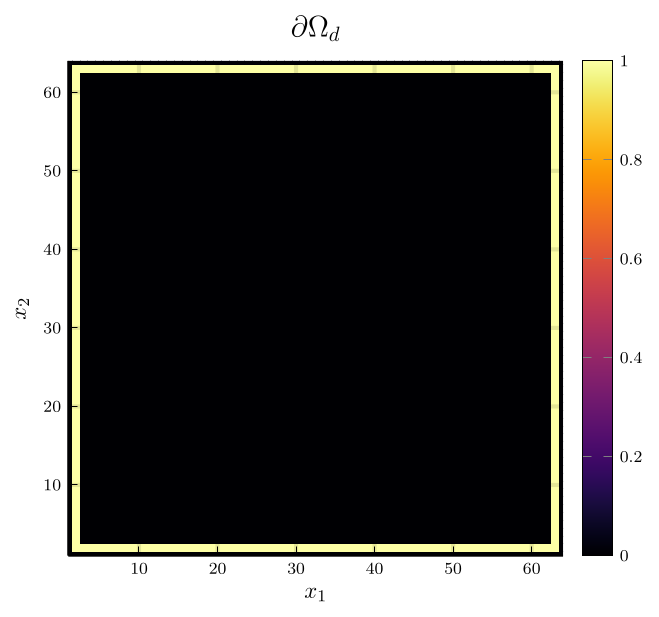
\includegraphics[width=.9\linewidth]{images/boundary.png}
\caption{\label{fig:boundary-square}Visualization of all grid-cells adjacent to the boundary \(\partial \Omega_{d}\) of a square domain}
\end{figure}



\begin{figure}[htbp]
\centering
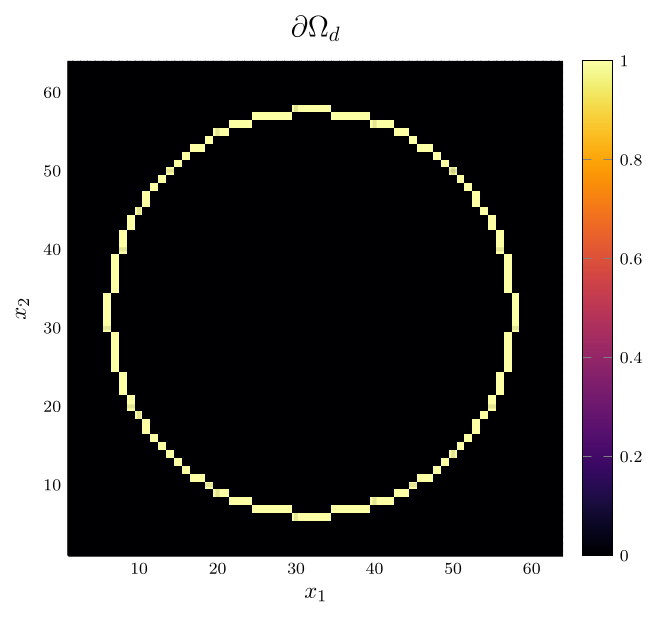
\includegraphics[width=.9\linewidth]{images/boundary-circle.png}
\caption{\label{fig:boundary-circle}Visualization of all grid-cells adjacent to the boundary \(\partial \Omega_{d}\) of a circular domain}
\end{figure}
\chapter{Numerical solver}
\label{sec:org1ac2f56}
Contrary to the solver proposed in \autocite{Ulmer_CHRelaxed_2024} we do not use a multi-grid Gauss-Seidel Solver to solve the linear system, instead we use a Jacobi solver, as this will eventually assist in parallelizing the computation.
Similar to \autocite{Ulmer_CHRelaxed_2024} we linearize \eqref{eq:second-order-adapted-ansatz} to
\begin{equation}
\begin{aligned}
\frac{\phi_{ij}^{n+1}}{\Delta t}  -  \nabla _d \cdot (G_{ij} \nabla_d \mu_{ij}^{n+\frac{1}{2}} ) &= \frac{ \phi_{ij}^n}{\Delta t}  \\
 \mu_{ij}^{n+\frac{1}{2}} - 2\phi_{ij}^{n+1} + \varepsilon^2  \nabla_d \cdot  (G_{ij} \nabla _d \phi_{ij}^{n+1} ) &=2\phi _{ij}^n - W'(\phi_{ij}^n)  - B_{ij}
\end{aligned}
\end{equation}
One may note, that after rearranging some terms leads to a linear system with a right-hand side which is exclusively dependent on the previous time step.
We use Jacobi's method to solve the resulting linear system given above, and the corresponding element wise representation of the same is given in the following.

Provided the \(mth\) Jacobi iteration has been computed, the \(m+1th\) iteration is computed by solving
\begin{equation}
\begin{aligned}
\frac{\phi_{ij}^{n+1,m+1}}{\Delta t}  -  \nabla _d \cdot (G_{ij} \nabla_d \mu_{ij}^{n+\frac{1}{2},m+\frac{1}{2}} ) &= \frac{ \phi_{ij}^{n}}{\Delta t}  \\
 \mu_{ij}^{n+\frac{1}{2},m} - 2\phi_{ij}^{n+1,m} + \varepsilon^2  \nabla_d \cdot  (G_{ij} \nabla _d \phi_{ij}^{n+1,m+\frac{1}{2}} ) + B_{ij} &=2\phi _{ij}^n - W'(\phi_{ij}^n)
\end{aligned}
\end{equation}
For \(\phi_{ij}^{n+1,m+1} , \mu_{ij}^{n+\frac{1}{2},m+1}\),
where \(\nabla _d \cdot (G_{ij} \nabla_d \mu_{ij}^{n+\frac{1}{2},m+\frac{1}{2}} )\) and \(\nabla_d \cdot  (G_{ij} \nabla _d \phi_{ij}^{n+1,m+\frac{1}{2}} )\) can be computed as follows. We use the results from the previous Jacoby step, \(m\), for values off the center. e.g.
\begin{equation}
\begin{aligned}
 \nabla _d \cdot (G_{ij} \nabla_d \phi_{ij}^{n+1,m+\frac{1}{2}} )  =&
\frac{1}{h^2}
\sum_{\Delta \in S} G_{ij + \frac{1}{2} \Delta}\phi_{ij + \Delta}^{n+1,m}  -
\left(
\sum_{\Delta \in S}  G_{ij+\frac{1}{2} \Delta}
\right)\phi_{ij}^{n+1,m+1}
\end{aligned}
\end{equation}
where \(S:= \{ (0,1) , (0,-1) , (1,0) , (-1,0)\}\).
Our implementation is done in julia to transmit the solution for each element in parallel on the GPU. In the following we described the complete implementation of the Jacobi's iteration.
\begin{Code}
\begin{Verbatim}
\color{EFD}\textcolor[HTML]{483d8b}{\textbf{@kernel}} \EFk{function} jacoby!(
    Φ,
    M,
    \textcolor[HTML]{483d8b}{\textbf{@Const}}(Ξ),
    \textcolor[HTML]{483d8b}{\textbf{@Const}}(Ψ),
    \textcolor[HTML]{483d8b}{\textbf{@Const}}(h),
    \textcolor[HTML]{483d8b}{\textbf{@Const}}(ε),
    \textcolor[HTML]{483d8b}{\textbf{@Const}}(Δt),
    \textcolor[HTML]{483d8b}{\textbf{@Const}}(iterations)
)
    I   = \textcolor[HTML]{483d8b}{\textbf{@index}}(Global, Cartesian)
    Id  = oneunit(I)
    Ids = CartesianIndices(M)
    Ix = CartesianIndex(\EFhn{1}, \EFhn{0})
    Iy = CartesianIndex(\EFhn{0}, \EFhn{1})
    \EFk{if} I in (Ids[\EFk{begin}]\EFt{+}Id:Ids[\EFk{end}]\EFt{-}Id)
        g = G(\EFhn{2} \EFt{*} I \EFt{+} Ix, Ids) \EFt{+} G(\EFhn{2} \EFt{*} I \EFt{+} Iy, Ids) \EFt{+} G(\EFhn{2} \EFt{*} I \EFt{-} Ix, Ids) \EFt{+} G(\EFhn{2} \EFt{*} I \EFt{-} Iy, Ids)
        a1 = \EFhn{1}\EFt{/}Δt
        a2 = \EFt{-}\EFhn{1}\EFt{*} ε\EFt{\char94{}}\EFhn{2}\EFt{/}h\EFt{\char94{}}\EFhn{2} \EFt{*} g  \EFt{-} \EFhn{2}
        b1 = \EFhn{1}\EFt{/}h\EFt{\char94{}}\EFhn{2} \EFt{*} g
        b2 = \EFhn{1}
        \EFk{for} \_ \EFk{=} \EFhn{1}:iterations

            Σμ = G(\EFhn{2} \EFt{*} I \EFt{+} Ix, Ids) \EFt{*} M[I\EFt{+}Ix] \EFt{+} G(\EFhn{2} \EFt{*} I \EFt{+} Iy, Ids) \EFt{*} M[I\EFt{+}Iy] \EFt{+} G(\EFhn{2} \EFt{*} I \EFt{-} Ix, Ids) \EFt{*} M[I\EFt{-}Ix] \EFt{+} G(\EFhn{2} \EFt{*} I \EFt{-} Iy, Ids) \EFt{*} M[I\EFt{-}Iy]

            Σϕ = G(\EFhn{2} \EFt{*} I \EFt{+} Ix, Ids) \EFt{*} Φ[I\EFt{+}Ix] \EFt{+} G(\EFhn{2} \EFt{*} I \EFt{+} Iy, Ids) \EFt{*} Φ[I\EFt{+}Iy] \EFt{+}G(\EFhn{2} \EFt{*} I \EFt{-} Ix, Ids) \EFt{*} Φ[I\EFt{-}Ix] \EFt{+}G(\EFhn{2} \EFt{*} I \EFt{-} Iy, Ids) \EFt{*} Φ[I\EFt{-}Iy]

            c1 = Ξ[I] \EFt{+} \EFhn{1}\EFt{/}h\EFt{\char94{}}\EFhn{2}   \EFt{*} Σμ
            c2 = Ψ[I] \EFt{-} ε\EFt{\char94{}}\EFhn{2}\EFt{/}h\EFt{\char94{}}\EFhn{2} \EFt{*} Σϕ

            \EFcd{\#} \EFc{stupid matrix solve}
            \textcolor[HTML]{483d8b}{\textbf{@inline}} Φ[I] = (c1\EFt{*}b2 \EFt{-} c2\EFt{*}b1) \EFt{/} (a1\EFt{*}b2 \EFt{-} a2\EFt{*}b1)
            \textcolor[HTML]{483d8b}{\textbf{@inline}} M[I] = (a1\EFt{*}c2 \EFt{-} a2\EFt{*}c1) \EFt{/} (a1\EFt{*}b2 \EFt{-} a2\EFt{*}b1)
            \EFcd{\#}
            \textcolor[HTML]{483d8b}{\textbf{@synchronize}}()
        \EFk{end}

    \EFk{end}
\EFk{end}
\end{Verbatim}
\end{Code}
\chapter{Numerical evaluation}
\label{sec:org75922b4}
the numerical investigations in this capter and the following are done with the following hyperparameters:
\begin{center}
\begin{tabular}{llll}
parameter & \(\varepsilon\) & \(h\) & \(\Delta t\)\\
\hline
value & \(8 * 10^{-5}\) & \(1*10^{-4}\) & \(1*10^{-4}\)\\
\end{tabular}
\end{center}
We set constant values for B\textsubscript{ij} on the boundary to begin with our evaluations.
One may note that C = 0 is equivalent to the no-flux condition of the original solver introduced in the Bachelor thesis. Now, as a preliminary verification step we set C = 0 as our first choice.
Consequently, for \(C = 0\), the interface lies orthogonal on the boundary (see Fig. \ref{fig:angle0}), which we expect for a CH solver with no-flux boundary conditions.
For \(B_{ij} \in \{-1,1\}\) we observed behavior connected to hydrophobic / hydrophilic substances on the boundary, where \(B_{ij}=1\) resulted in the one phase pearling off the boundary, while the other seemed attracted. These certainly leads to the apparent contact angles of 180° and 0° respectively. Using \(B_{ij} = -1\) results in the opposite behavior.

\begin{figure}[htbp]
\centering
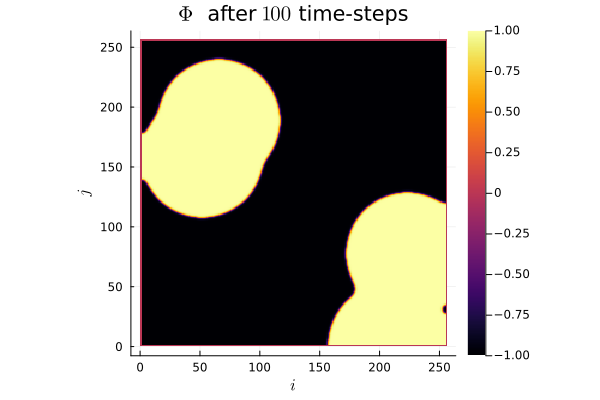
\includegraphics[width=.9\linewidth]{images/baseline.png}
\caption{\label{fig:angle0}Phase-field \(\phi\) after 100 time-steps with \(C=0\) emulating no-flux boundary.}
\end{figure}

We show, that our solver is stable for values \(C \neq 0\). In Fig. \ref{fig:angle1} we employ a constant value of \(C=1\) and observe the phase corresponding to \(\phi = 1\) puling away from the boundary. The contact angle between phase 1 and the boundary approaches 180° i.e. the interface runs parallel to the boundary.
\begin{figure}[htbp]
\centering
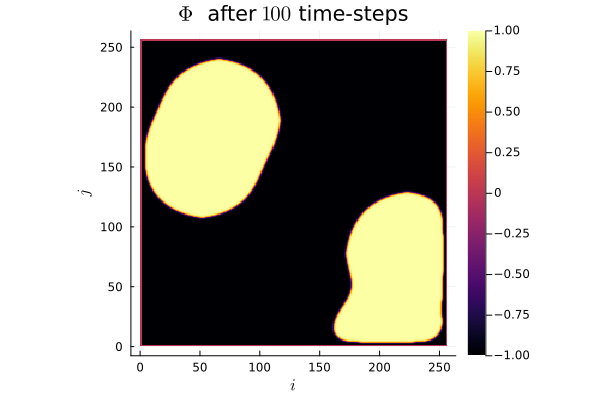
\includegraphics[width=.9\linewidth]{images/angle1.png}
\caption{\label{fig:angle1}phase-field   \(\phi\) after 100 time steps with \(C=1\)}
\end{figure}


In Fig. \ref{fig:angle-1} we try the reverse situation, and consequently we observe the corresponding behavior. When using a value of \(C=-1\) we observe opposite behavior relative to the case in Fig. \ref{fig:angle1}. Where the contact angle on the boundary lies at 0°, the interface runs parallel to the boundary again.
\begin{figure}[htbp]
\centering
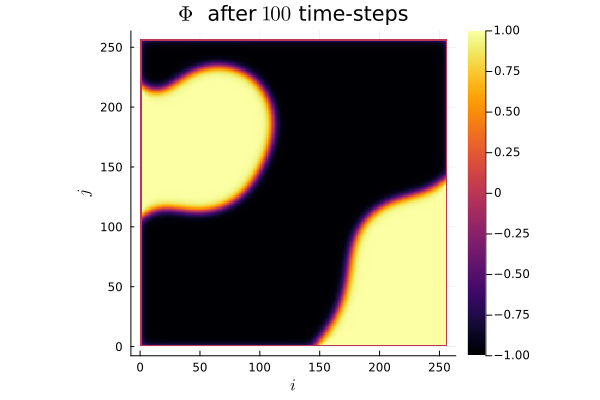
\includegraphics[width=.9\linewidth]{images/angle-.png}
\caption{\label{fig:angle-1}phase-field \(\phi\) after 100 time-steps with \(C=-1\)}
\end{figure}

The most interesting behavior are noted for values between \((-1,1)\), where we observe the contact angle of the interface at the boundary changes from parallel 0° to parallel 180°.
\begin{figure}[htbp]
\centering
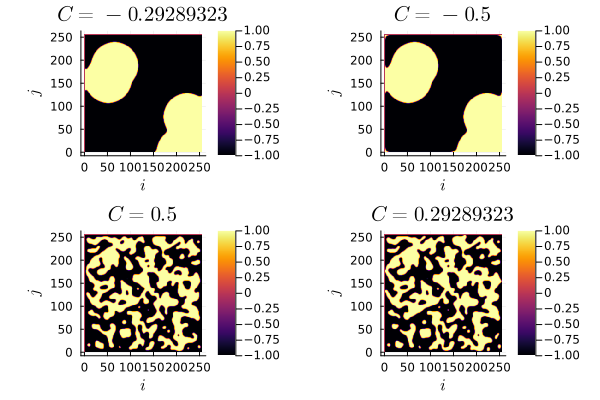
\includegraphics[width=.9\linewidth]{images/angle-sqrt(2).png}
\caption{\label{fig:angle-multiple}phase-field \(\phi\) after 500 time-steps with \(C \in \{-1 + \frac{\sqrt{2}}{2} , -0.5 , 0.5 , 1 - \frac{\sqrt{2}}{2} \}\)}
\end{figure}
\chapter{Numerical evaluation on a circle}
\label{sec:org7ce30bd}
The original solver presented in \autocite{SHIN20117441} was able to solve the CH equation on arbitrary domains. Since the addition of our boundary function depends solely on the characteristic function of the discrete domain, we are able to use our approach on different domains, by providing a different characteristic function. We present the results of which in this chapter.
To show the behavior of the CH solver in Fig. \ref{fig:angle0c}, we first employ no-flux boundary conditions on a circular domain. We observe the interface perpendicular on the boundary, as we expect.

\begin{Code}
\begin{Verbatim}
\color{EFD}\textcolor[HTML]{483d8b}{\textbf{@inline}} \EFk{function} \EFf{G}(I\EFt{::CartesianIndex} , Ids\EFt{::CartesianIndices})\EFt{::Float32}
    \textcolor[HTML]{483d8b}{\textbf{@inline}} r  = Ids[\EFk{end}] \EFt{-} I
    m = maximum(Tuple(Ids[\EFk{end}]))
    \EFk{if} norm(Tuple(r)) \EFt{<} \EFhn{0.8} \EFt{*} m
        \EFk{return} \EFhn{1.}
        \EFk{end}
    \EFk{return} \EFhn{0.}
\EFk{end}

h\EFt{::Float32} = \EFhn{3}f\EFt{-}\EFhn{4}
Δt\EFt{::Float32} = \EFhn{1e-4}
ε\EFt{::Float32} = \EFhn{2e-4}
\EFf{W′}(x) = \EFt{-}x \EFt{*} (\EFhn{1} \EFt{-} x\EFt{\char94{}}\EFhn{2})
\end{Verbatim}
\end{Code}

\phantomsection
\label{}
\begin{verbatim}
W′ (generic function with 1 method)
\end{verbatim}



\begin{figure}[htbp]
\centering
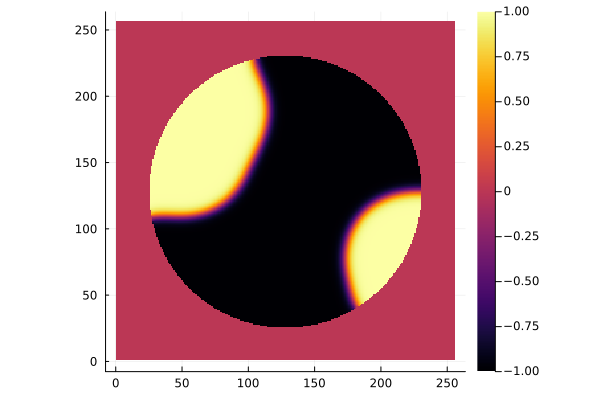
\includegraphics[width=.9\linewidth]{images/angle0c.png}
\caption{\label{fig:angle0c}\(\phi\) after 100 time steps on a circular domain with no-flux boundary-conditions after 100 time steps on a circular domain with no-flux}
\end{figure}



The results we observe in Fig. \ref{fig:angle1c} are similar to the results on a square domain in Fig. \ref{fig:angle1}. The contact angle is 180° i.e. the interface does not touch the boundary and runs parallel to it.
\begin{figure}[htbp]
\centering
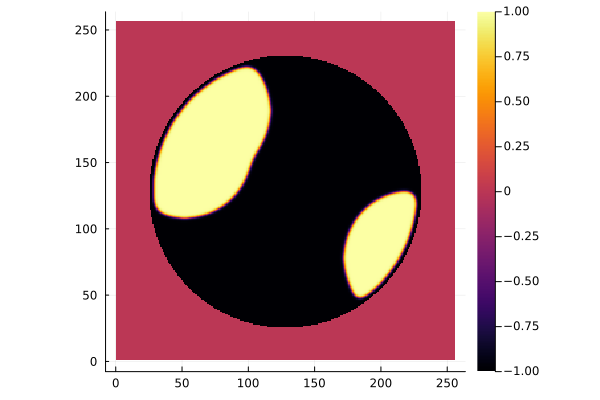
\includegraphics[width=.9\linewidth]{images/anfle1c.png}
\caption{\label{fig:angle1c}phase-field \(\phi\) after 100 time-steps with \(C=1\)}
\end{figure}

The results for \(C=-1\) in Fig. \ref{fig:angle-1c} on the circular domain, are similar to the results in Fig. \ref{fig:angle-1} on the square domain as well, where the interface touches the boundary and runs parallel with a contact angle of 0°.
\begin{figure}[htbp]
\centering
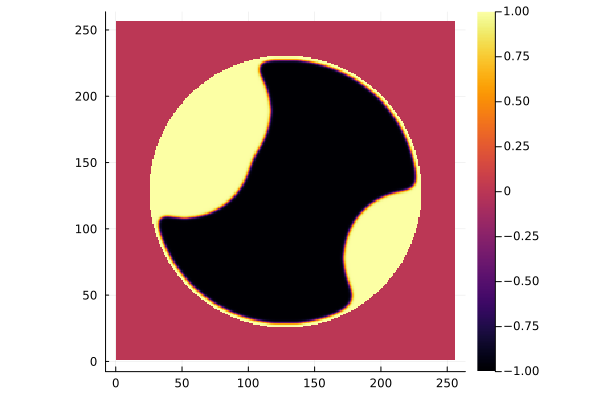
\includegraphics[width=.9\linewidth]{images/angle-1c.png}
\caption{\label{fig:angle-1c}Phase-field \(\phi\) after 100 time-steps with \(C=-1\)}
\end{figure}

When evaluating intermediate contact angles in Fig. \ref{fig:angle-multiplec}, the results are similar to the square domain again, however, especially for shallow angles, we observe some artifacts of one phase appearing in places where previously was none. We observe similar behavior on square domains only in the corners, i.e. points where the boundary has high curvature. Note that this effect can be circumvented with different values for \(\varepsilon\) howeverthis has an effect on the boundary angle, that we did not investigate.
\begin{figure}[htbp]
\centering
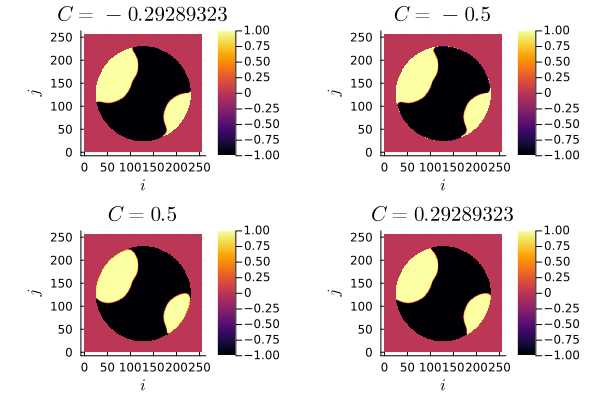
\includegraphics[width=.9\linewidth]{images/angle-multiplec.png}
\caption{\label{fig:angle-multiplec}Phase-field \(\phi\) after 500 time-steps with \(C \in \{-1 + \frac{\sqrt{2}}{2} , -0.5 , 0.5 , 1 - \frac{\sqrt{2}}{2} \}\) on a circular domain.}
\end{figure}



When using random initial phase-fields, the results look the comparable to the square domain, and exhibit the for the CH equation expected behavior, whereas time goes on, the many small parts coalesce into larger parts.
\chapter{Angle}
\label{sec:org87a873f}
We calculate the angle using the folowing hyperparameters
\begin{center}
\begin{tabular}{llll}
parameter & \(\varepsilon\) & \(h\) & \(\Delta t\)\\
\hline
value & \(2 * 10^{-5}\) & \(1*10^{-4}\) & \(1*10^{-4}\)\\
\end{tabular}
\end{center}
In previous experiments we noted that the angle of the interface changes with different input parameters. While we do not have a mathematical derivation of this relation, we aim to provide numerical insight in this chapter. We calculate this angle using the gradient of the phase-field \(\nabla \phi_{ij}\) and the normal of our domains' boundary.
\begin{align}
\label{eq:1}
\frac{\nabla_d \phi_{ij} \cdot \mathbf{n}_{ij}}{\|\nabla_{d} \phi_{ij}\|} &= \cos(\theta),& \text{where}\,&\, \phi_{ij} \in \partial\Omega_{d}
\end{align}
For a single point \(\vec{x}_{ij}\) on the interface and near the boundary. Since we need a finite difference to evaluate \eqref{eq:1}, we do not select a point directly on the boundary and since we need a point on the interface, where \(\nabla \phi_{ij}\) is large, we calculate the angle at
\begin{equation}
\label{eq:2}
P_{ij} = arg\max_{\vec{x}_{ij}} \nabla \phi_{ij} \qquad \text{where} \quad \phi_{ij} \in \partial \Omega
\end{equation}
\section{Circle}
\label{sec:org9915123}
The normal of the circular domain in our second example is
\begin{equation}
\label{eq:3}
\mathbf{n}_{ij} := \mathbf{n}(\vec{x}_{ij}) = \frac{\vec{c} - \vec{x}_{ij}}{\| \vec{c} - \vec{x}_{ij}\|}
\end{equation}
Where \(\vec{c}\) is the center of the domain.
In Fig. \ref{fig:angle-on-circle} we present the results of a calculated angle, together with the normals and the point it is calculated from.
\begin{figure}[htbp]
\centering
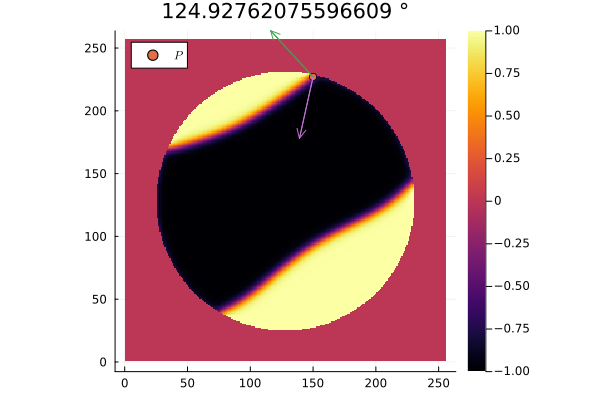
\includegraphics[width=.9\linewidth]{images/angle-circle.png}
\caption{\label{fig:angle-on-circle}Plot of the boundary and surface normals on a circular domain}
\end{figure}


The method we use to calculate the interface-boundary angle is not stable under small changes in \(C\) as seen in  Fig. \ref{fig:angle-table} this is unsurprising, since the selection criterion for the point, where we calculate the angle is prone to change as the maximum derivative of the phase-field is approximately the same everywhere on the phase-field. To combat this effect, we chose the point to evaluate at once for all iterations. This however only works if the interface doesn't move from the point selected. The results in Fig. \ref{fig:angle-table} shows, that the contact angle is related to the value we use for \(C\). Since the other hyperparameters (\(\varepsilon\) and \(h\)) may have an effect on the angel as well, we cannot give an exact relation.

\begin{figure}[htbp]
\centering
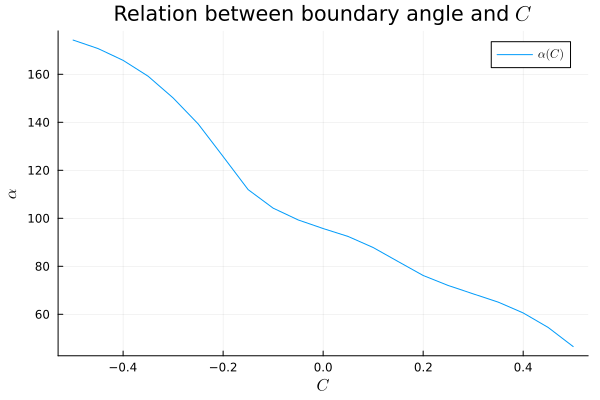
\includegraphics[width=.9\linewidth]{images/angle-values-circle.png}
\caption{\label{fig:angle-table}value for \(C\) and corresponding angle \(\alpha\) after 200 time-steps}
\end{figure}
\section{Square}
\label{sec:orgdfcdecb}
The normal vector on a square domain is a little bit more complicated than the normal for the circle. In this case we use the normal
\begin{equation}
\label{eq:9}
\mathbf{n}_{ij} = \mathbf{n}(\vec{x}_{ij}) = \max(\vec{c} - \vec{x}_{ij}) e_{\argmax_{i,j}(\vec{c} - \vec{x}_{ij})}
\end{equation}
The angle on a square domain is presented in Fig. \ref{fig:angle-on-square}
\begin{figure}[htbp]
\centering
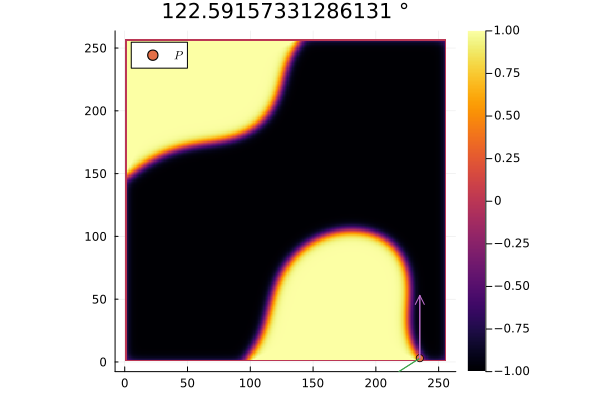
\includegraphics[width=.9\linewidth]{images/angle-square.png}
\caption{\label{fig:angle-on-square}Plot of the boundary and surface normals on a circular domain}
\end{figure}



The relation between the contact angle and \(C\), as seen in Fig. \ref{fig:angle-table-square} is about the same as in the circular domain
\begin{figure}[htbp]
\centering
\includegraphics[width=.9\linewidth]{images/angle-values-square.png}
\caption{\label{fig:angle-table-square}value for \(\theta\) and corresponding angle \(\alpha\) after 200 time-steps}
\end{figure}
\chapter{Summary and outlook}
\label{sec:orgbd2a86c}
In this project we examined a numerical model of the CH equation, with simple Neumann boundary conditions. We introduced a simplified version of the solver used in \autocite{Ulmer_CHRelaxed_2024} and derived from \autocite{SHIN20117441}. Which due to GPU acceleration is significantly faster on our available hardware. We have shown a simple Neumann boundary approach that runs stable on both tested domains. The approach introduced by us is able to freely affect the angle of the phase interface on the boundary, The results of which we have shown on a circular and square domain. We introduced a rudimentary method to calculate the contact angle programmatically however we acknowledge that the results are unreliable. Further research would require a more consistent approach. One such method may be a filter that averages the angle calculation over more than one point, another should be a consistent selection of the point of interest, as the current approach cannot guaranty that the same (or a similar) point is selected if the input parameters change slightly.

Further research may concern itself, with the following topics. First and foremost, we observed inconsistent behavior when changing the hyperparameters \(\varepsilon\) and grid-size \(h\). However, the methods we used for evaluation were inconsistent at best. Due to the aforementioned unpredictability in the angle calculation the resulting data series was erratic and no trends where apparent. Further research would require investigation of those effects on the boundary. Additionally, in our bachelor thesis, which served as preliminary work to this project, we investigated an analytical relaxation. The solver used therein for the relaxed problem is compatible with the boundary approach introduced herein. Initial tests with the solver for the relaxed system where promising, and further research may investigate those results.


\printbibliography
\end{document}
